Presta mucha atención a estas notas, de seguro aprenderás cosas muy novedosas que servirán para elevar tu cultura matemática.

i) En todo triángulo hay para cada lado una altura, una mediana, una mediatriz y para cada ángulo una bisectriz. cada una de estas rectas concurren en un punto llamado: ortocentro, baricentro, circuncentro e incentro $(H, G, T, I)$

\vspace{0.5cm}
$\cdot\hspace{0.05cm}\text{-}$ alturas

\noindent\parbox[][][t]{.3\linewidth}{
    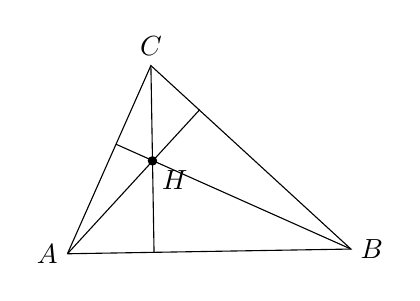
\begin{tikzpicture}
      \coordinate [label=left:$A$] (A) at (0,0);
      \coordinate [label=right:$B$] (B) at (3.6,0.06);
      \coordinate [label=above:$C$] (C) at (1.06,2.39);
      \coordinate [label=below right:$H$] (H) at (1.08,1.18);
      
      \coordinate (P) at (1.68,1.83);
      \coordinate (Q) at (0.62,1.39);
      \coordinate (R) at (1.1,0.02);
      
      \filldraw (H) circle[radius=1.5pt];
      \draw (A) -- (B) -- (C) -- (A);
      \draw (B) -- (Q);
      \draw (C) -- (R);
      \draw (A) -- (P);
      
      \tkzMarkRightAngle(H,R,B);
      \tkzMarkRightAngle(H,P,C);
      \tkzMarkRightAngle(H,Q,A);
    \end{tikzpicture}
}
\parbox[][][t]{.05\linewidth}{\hspace{.03\linewidth}}
\parbox[][][t]{.65\linewidth}{
 Segmentos que ``parten'' de cada vértice y ``caen'' perpendicularmente en los lados opuestos. Vemos que $H$ es un pinto interior del triángulo si este es acutángulo, pero si es un triángulo obtusángulo entonces $H$ es un punto exterior y si el triángulo es rectángulo entonces $H$ coincide con el vértice del ángulo recto
}

\vspace{0.5cm}
$\cdot\hspace{0.05cm}\text{-}$ medianas

\noindent\parbox[][][t]{.3\linewidth}{
    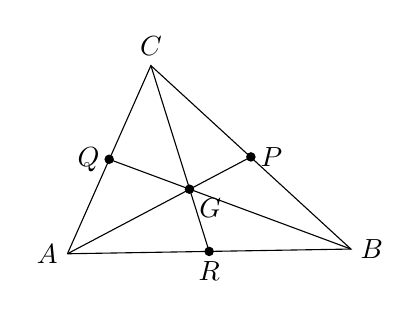
\begin{tikzpicture}
      \coordinate [label=left:$A$] (A) at (0,0);
      \coordinate [label=right:$B$] (B) at (3.6,0.06);
      \coordinate [label=above:$C$] (C) at (1.06,2.39);
      \coordinate [label=below right:$G$] (G) at (1.55,0.82);
      
      \coordinate [label=left:$Q$] (Q) at (0.53,1.2);
      \coordinate [label=right:$P$] (P) at (2.33,1.23);
      \coordinate [label=below:$R$] (R) at (1.8,0.03);
      
      \filldraw (G) circle[radius=1.5pt];
       \filldraw (P) circle[radius=1.5pt];
      \filldraw (Q) circle[radius=1.5pt];
      \filldraw (R) circle[radius=1.5pt];
      \draw (A) -- (B) -- (C) -- (A);
      \draw (B) -- (Q);
      \draw (C) -- (R);
      \draw (A) -- (P);
      \tkzMarkSegment[mark=|||](A,Q);
      \tkzMarkSegment[mark=|||](Q, C);
      \tkzMarkSegment[mark=||](C,P);
      \tkzMarkSegment[mark=||](P, B);
      \tkzMarkSegment[mark=|](B,R);
      \tkzMarkSegment[mark=|](R, A);
    \end{tikzpicture}
    
}
\parbox[][][t]{.05\linewidth}{\hspace{.03\linewidth}}
\parbox[][][t]{.65\linewidth}{
 Segmentos que ``parten'' de cada vértice y ``caen'' en el punto medio de cada lado. Vemos que $G$ siempre va a ser un punto interior del triángulo
 \begin{itemize}
     \item[* -] $\overline{AG} = 2\overline{GP}$, $\overline{BG} = 2\overline{GQ}$, $\overline{CG} = 2\overline{GR}$
     \item[-] $\overline{PQ}$, $\overline{QR}$ y $\overline{RP}$ son las paralelas medias de $\overline{AB}$, $\overline{BC}$ y $\overline{CA}$ respectivamente
     \item[* -] Los $\triangle AGR$, $\triangle BGR$, $\triangle BGP$, $\triangle CGP$, $\triangle CGQ$ y $\triangle AGQ$ tienen la misma área
 \end{itemize}
}

\vspace{0.5cm}
$\cdot\hspace{0.05cm}\text{-}$ mediatrices

\noindent\parbox[][][t]{.3\linewidth}{
    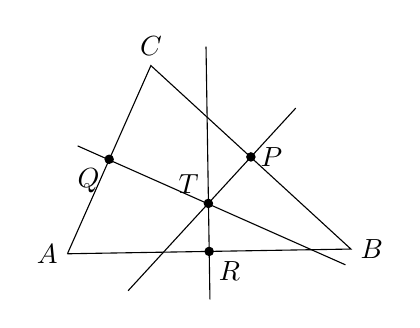
\begin{tikzpicture}
      \coordinate [label=left:$A$] (A) at (0,0);
      \coordinate [label=right:$B$] (B) at (3.6,0.06);
      \coordinate [label=above:$C$] (C) at (1.06,2.39);
      \coordinate [label=above left:$T$] (T) at (1.79,0.64);
      
      \coordinate [label=below left:$Q$] (Q) at (0.53,1.2);
      \coordinate [label=right:$P$] (P) at (2.33,1.23);
      \coordinate [label=below right:$R$] (R) at (1.8,0.03);
      
      \filldraw (T) circle[radius=1.5pt];
      \filldraw (P) circle[radius=1.5pt];
      \filldraw (Q) circle[radius=1.5pt];
      \filldraw (R) circle[radius=1.5pt];
      \draw (A) -- (B) -- (C) -- (A);
      \draw (3.53, -0.14) -- (0.13,1.37);
      \draw (1.76, 2.63) -- (1.81,-0.58);
      \draw (0.77,-0.47) -- (2.9, 1.85);
      
      \tkzMarkRightAngle(T,R,B);
      \tkzMarkRightAngle(T,P,C);
      \tkzMarkRightAngle(T,Q,A);
    \end{tikzpicture}
    
}
\parbox[][][t]{.05\linewidth}{\hspace{.03\linewidth}}
\parbox[][][t]{.65\linewidth}{
 Rectas perpendiculares a cada lado que pasan por el punto medio de cada lado. Vemos que $T$ es un punto interior del triángulo si este es acutángulo, pero si es obtusángulo entonces $T$ es un punto exterior y si el triángulo es rectángulo entonces $T$ coincide con el punto medio de la hipotenusa
 
}

\begin{itemize}
     \item[-] $T$ coincide con el centro de la circunferencia circunscrita al triángulo
     \item[-] $\overline{GH} = 2\overline{GT}$ (recuerda que $G$ es el baricentro y $H$ el ortocentro)
     \item[-] Los puntos $H$, $G$, $T$ son alineados (Recta de Euler)
     \item[-] Todo punto situado en la mediatriz de cualquier lado equidista de los extremos del lado
 \end{itemize}
 
 \vspace{0.5cm}
 $\cdot\hspace{0.05cm}\text{-}$ bisectrices

\noindent\parbox[][][t]{.3\linewidth}{
    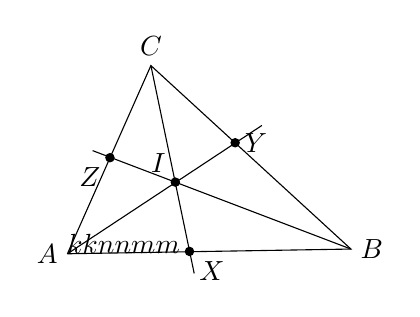
\begin{tikzpicture}[
      my angle/.style={
        every pic quotes/.append style={text=black},
        draw=white,
        draw opacity=0,
        angle radius=1cm
      }]
      \coordinate [label=left:$A$] (A) at (0,0);
      \coordinate [label=right:$B$] (B) at (3.6,0.06);
      \coordinate [label=above:$C$] (C) at (1.06,2.39);
      \coordinate [label=above left:$I$] (I) at (1.37,0.91);
      
      \coordinate [label=below left:$Z$] (Z) at (0.54,1.22);
      \coordinate [label=right:$Y$] (Y) at (2.13,1.41);
      \coordinate [label=below right:$X$] (X) at (1.55,0.03);
      
      \filldraw (I) circle[radius=1.5pt];
      \filldraw (Y) circle[radius=1.5pt];
      \filldraw (Z) circle[radius=1.5pt];
      \filldraw (X) circle[radius=1.5pt];
      \draw (A) -- (B) -- (C) -- (A);
      \draw (C) -- (1.61,-0.25);
      \draw (A) -- (2.47,1.63);
      \draw (B) -- (0.32,1.31);
     
      \tkzLabelAngle[pos=0.5](I,C,Y){$k$}; 
      \tkzLabelAngle[pos=0.5](A,C,I){$k$};  
       \tkzLabelAngle[pos=0.5](X,A,I){$n$}; 
      \tkzLabelAngle[pos=0.5](I,A,Z){$n$};
       \tkzLabelAngle[pos=0.8](C,B,I){$m$}; 
      \tkzLabelAngle[pos=0.8](I,B,X){$m$};
    \end{tikzpicture}
}
\parbox[][][t]{.05\linewidth}{\hspace{.03\linewidth}}
\parbox[][][t]{.65\linewidth}{
 Son rectas que dividen a cada ángulo del triángulo en dos ángulos de igual amplitud. vemos que $I$ siempre va a ser un punto interior del triángulo
 \begin{itemize}
     \item[* -] $I$ coincide con el centro de la circunferencia inscrita en el triángulo
     \item[* -] $\overline{CX}^2 = \overline{AC} \cdot \overline{CB} - \overline{AX} \cdot \overline{XB}$, análogamente para $\overline{AY}$ y $\overline{BZ}$
     \item[* -] $\overline{AI}:\overline{BI}=\overline{AX}:\overline{BX}$, $\overline{BI}:\overline{CI}=\overline{BY}:\overline{CY}$, $\overline{CI}:\overline{AI}=\overline{CZ}:\overline{AZ}$
     \item[* -] Todo punto situado en la bisetriz de cualquier ángulo equidista de los lados que determinan al ángulo
 \end{itemize}
}

\vspace{0.5cm}
\noindent2) Particularidades importantes

Vea que los cuatro putos y 4 rectas notables no tienen porqué coincidir pero en un triángulo isósceles, las 4 rectas notables referidas a las base coinciden y los cuatro pintos notables serían puntos alineados sobre ellas.

Ahora el triángulo equilátero ``esconde'' otras ``cositas'' que hacen de él un polígono muy interesante, veamos...
\begin{itemize}
    \item[-] Para cada lado las cuatro rectas notables coinciden
    \item[-] Los cuatro pntos notables coinciden también
\end{itemize}

Esto genera resultados a destacar, veamos...
\begin{equation*}
    \begin{aligned}
        \text{Sean } a &\rightarrow \text{longitud de los lados}\\
        h &\rightarrow \text{altura de los lados}\\
        S &\rightarrow \text{área del triángulo}\\
        r &\rightarrow \text{radio de la circunferencia inscrita}\\
        R &\rightarrow \text{radio de la circunferencia circunscrita}\\
    \end{aligned}
\end{equation*}

\hfill$* \Longrightarrow$\hfill$h= R + r$\hfill$R = 2r$\hfill$h=\dfrac{\sqrt{3}}{2}a$\hfill$S = \dfrac{a^2\sqrt{3}}{4}$\hfill

Vea que es suficiente conocer cualesquiera dos de estas variables para poder conocer el valor de las otras 3.

\vspace{0.5cm}
\noindent Otras notas de interés
\begin{itemize}
    \item[* -] Sean $b_a$, $b_b$, $b_c$ $\rightarrow$ longitud de las bisectrices de $a$, $b$ y $c$ y $p \rightarrow$ semiperímetro del triángulo
    \item[] $\Longrightarrow b_a=\dfrac{2}{b+c}\sqrt{bc(p-a)}$ y así con $b_b$ y $b_c$
    \item[* -] Sean $m_a$, $m_b$ $m_c$ $\rightarrow$ longitud de las medianas de los lados $a$, $b$ y $c$
    \item[]$\Longrightarrow m_a = \dfrac{1}{2}\sqrt{2(b^2 + c^2)- a^2}$ y así con $m_b$ y $m_c$
    \item[* -] Sean $h_a$, $h_b$, $h_c$ $\rightarrow$ longitud de las alturas de los lados$a$, $b$ y $c$
    \item[] $\Longrightarrow h_a = \dfrac{2}{a}\sqrt{p(p-a)(p-b)(p-c)}$ y así con $h_b$ y $h_c$
    \item[* -] Sean $K$ circuncentro, $I$ incentro, $R$ circunradio y $r$ inradio
    \item[] $\Longrightarrow (KI)^2 = R^2 - 2Rr$ (fórmula de Euler)
    \item[* -] Simedianas de un triángulo: En $\triangle ABC$: $\overline{AM}$ mediana, $\overline{AD}$ bisectriz $\Longrightarrow \overline{AX}$ es simediana de $\overline{BC}$ si $\overline{AD}$ biseca al $\measuredangle XAM$ y se cumple:
    \item[] $\dfrac{\overline{XB}}{\overline{XC}}=\dfrac{\overline{AB}^2}{\overline{AC}^2}$ El punto donde las tres simedianas se cortan se llama Punto de Lemoine
    \item[* -] Los segmentos trazados desde cada vértice de un triángulo dado con el vértice más alejado del triángulo equilátero trazado exteriormente a dicho triángulo sobre el lado opuesto al triángulo dado son iguales. Estos tres segmentos se cortan en un punto llamado: Punto de Fermat 
\end{itemize}


\vspace{0.5cm}
\noindent4, 5, 6, ... pueden ser sugerencias de los amigos de la matemática a estos temas

\vspace{0.5cm}
\begin{center}
    \textbf{Las notas marcadas con * deben ser demostradas}
\end{center}

